\documentclass{article}
\usepackage[widepage]{repsty}
\usepackage[utf8]{inputenc}
\usepackage[T1]{fontenc}
\usepackage[english, russian]{babel}
\usepackage{subcaption}

\newcommand{\Kmagic}{270.0092} %% best estimate by Sx component was 270.0092362, but at that point I didn't observe Sz turning from 1, and besides, our rest mass is defined down to the 4th digit

\begin{document}

\title{Анализ декогеренции в FS (BNL) структуре со случайными наклонами E+B элементов}
\maketitle

\section{Введение. FS структура}

Структура с замороженным спином (FS) --- это накопительное кольцо для эскперимента по поиску ЭДМ в котором спин частицы пучка непрерывно сонаправлен с вектором импульса частицы. Такое возможно для некоторых частиц, таких как дейтрон, только при некоторых ``магических'' значениях кинетической энергии. Для дейтрона, эта энергия находится в районе 270 МэВ.

В этой работе анализируется структура с элементами с совмещёнными E+B полями, расположенными в арках кольца. 

\section{Дизайн симуляции}
Симуляция была проведена с использованием программы COSY Infinity; использовалось отображение структуры в 3d, построенное до 5го порядка разложения Тейлора. E+B элементы моделируются неоднородными Вин-вильтрами (WC), наклонёнными на случайный угол вокруг оптической оси. Рассматриваются два случая: распределение углов имеет
\begin{inparaenum}[1)]
\item нулевое ожидание, и
\item ожидание $0.5\cdot 10^{-4}$ радиан.
\end{inparaenum}
В обоих случаях, стандартное отклонение распределения углов --- $10^{-4}$ радиан.

Три ансамбля по 15 частиц, плюс квази-референсная (с начальным отклонением по оси x $10^{-6}$ мм) пропущены через структуру на $10^6$ оборотов:
\begin{inparaenum}[1)]
\item частицы с начальным отклонением в x-направлении в диапазоне $\pm 7$ мм,
\item с таким же разбросом а y-направлении,
\item с разбросом по энергии $\pm 7\cdot 10^{-4} \Delta K/K$, где $K$ --- референсная кинетическая энергия (\Kmagic МэВ).
\end{inparaenum}

Наилучшая оценка величины кинетической энергии, найденная для этой структуры --- \Kmagic МэВ. Результаты симуляции не чувствительны к более точным подстройкам. При этой энергии, прецессия спина в горизонтальной плоскости всё ещё наблюдается в системе координат, связанной с пучком, то есть условие замороженности спина не выполняется. (За 250,000 оборотов, приблизительно четверть секунды, $S_x$ компонента спина растёт на $10^{-5}$.) По этой причине, мы корректируем спин-векторы частиц ансамбля в плоскости x-z после каждого оборота, чтобы симулировать эффект замороженности спина. Корректировака выполняется путём поворота спин-векторов частиц ансамбля на линию изначального направления спина ($\vec S_0: S_x = 0,~ S_z = 1$) на их средний угол отклонения от этого направления. Таким образом, декогеренция в горизонтальной плоскости предполагается незатронутой. (Выполнение условия замороженности спина имеет значительное влияния на прецессию в вертикальной плоскости, что наблюдалось в симуояциях при отключении коррекции.) Если средний угол меньше $\pi/2$, поворот осуществляется в направлении $+\vec S_0$, иначе, в направлении $-\vec S_0$. Это сделано чтобы не вмешиваться в прецессию в вертикальной плоскости: когда вертикальная компонента спина $S_y$ растёт, его проекция на плоскость x-z находится в первом и четвёртом квадрантах, а когда уменьшается --- в квадрантах 3 и 4. Если бы направление коррекции всегда было $+\vec S_0$, спин бы остановился на положении $\vec S = (0, 1, 0)$, и перестал бы прецессировать в обеих плоскостях x-z и z-y.

Далее рассматривается декогеренция в горизонтальной и вертикальной плоскостях.

\section{Декогеренция в горизонтальной плоскости}

\begin{figure}[!ht]
  \centering
  \begin{subfigure}[b]{1\textwidth}
    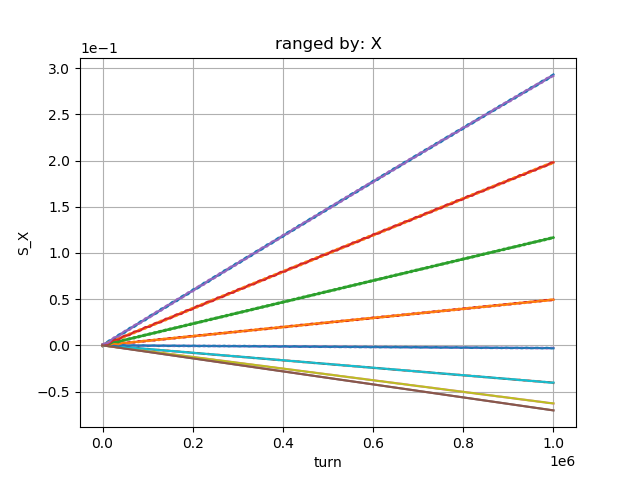
\includegraphics{img/S_X_vs_iteration_1_ranged_X}
  \end{subfigure}
  \begin{subfigure}[b]{1\textwidth}
    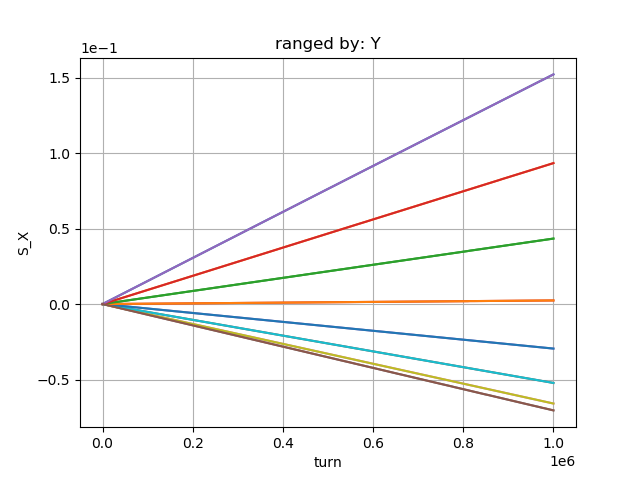
\includegraphics{img/S_X_vs_iteration_1_ranged_Y}
  \end{subfigure}
\end{figure}
\begin{figure}[!ht]\ContinuedFloat
  \begin{subfigure}[b]{1\textwidth}
    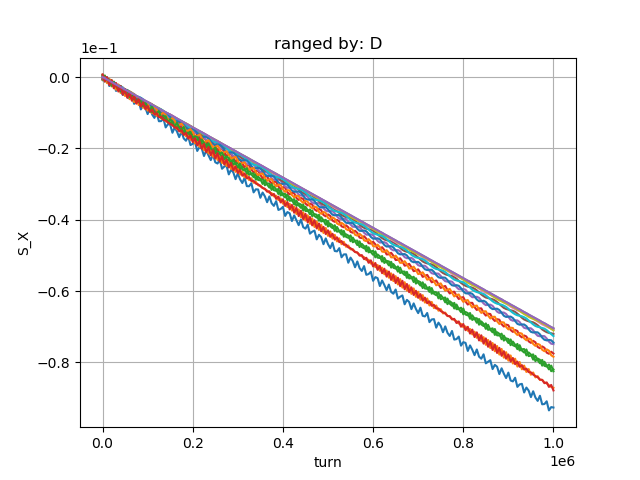
\includegraphics{img/S_X_vs_iteration_1_ranged_D}
  \end{subfigure}
  \caption{Рост горизонтальной компоненты спина}
\end{figure}

\section{Декогеренция в вертикальной плоскости}

\begin{figure}[!ht]
  \centering
  \begin{subfigure}[b]{1\textwidth}
    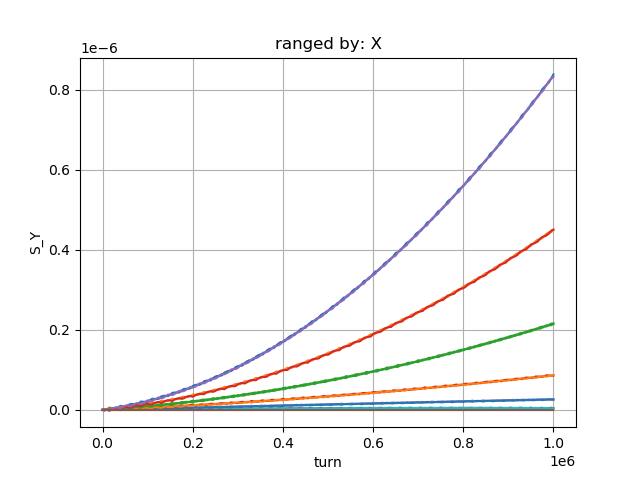
\includegraphics{img/S_Y_vs_iteration_1_ranged_X}
  \end{subfigure}
  \begin{subfigure}[b]{1\textwidth}
    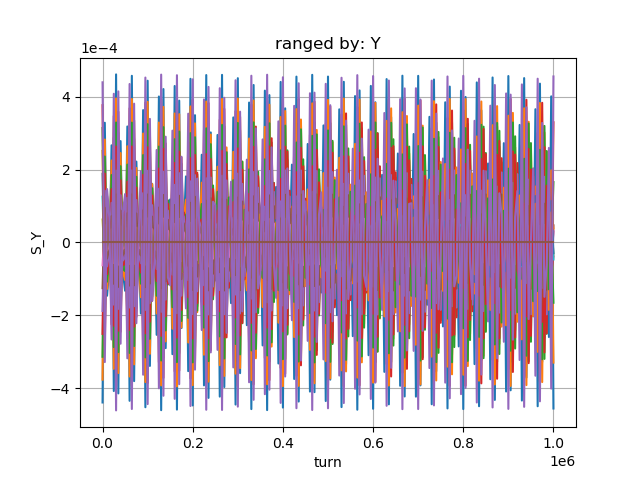
\includegraphics{img/S_Y_vs_iteration_1_ranged_Y}
  \end{subfigure}
\end{figure}
\begin{figure}[!ht]\ContinuedFloat
  \begin{subfigure}[b]{1\textwidth}
    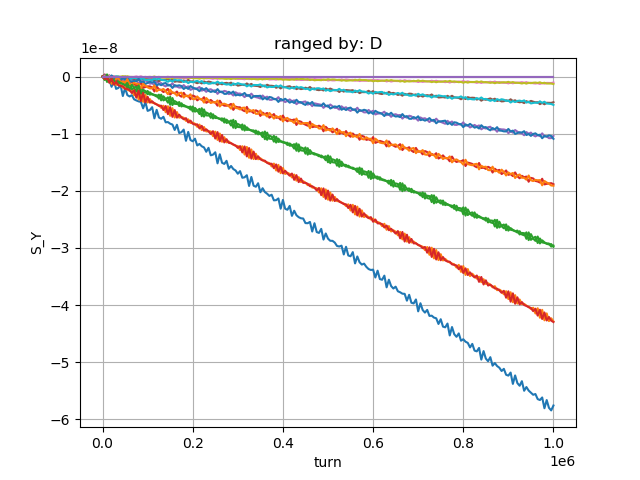
\includegraphics{img/S_Y_vs_iteration_1_ranged_D}
  \end{subfigure}
  \caption{Рост вертикальной компоненты спина}
\end{figure}


\end{document}

